%!Mode:: "TeX:UTF-8"
\documentclass[a4paper,11pt,UTF8]{ctexart}

\usepackage{indentfirst} %缩进
\usepackage{xeCJK}    %使用系统字体
\usepackage{fancyhdr} %自定义页眉页脚
\pagestyle{empty}                   %不设置页眉页脚
\usepackage{amsmath, amsthm, amssymb, amsfonts} %数学公式
\usepackage[a4paper,left=3cm,right=3cm,top=3cm,bottom=3cm]{geometry}
%\usepackage[tmargin=1in,bmargin=1in,lmargin=1.25in,rmargin=1.25in]{geometry}.
\usepackage{booktabs} %插入表格
\usepackage[section]{placeins} %避免浮动
\usepackage{listings} %插入代码
\usepackage{ctex}     %中文宏包
\usepackage[svgnames, table]{xcolor} %彩色表格
\usepackage{algorithm}          %伪代码
\usepackage{algorithmicx}
\usepackage{algpseudocode}
\usepackage{algorithm,algpseudocode,float}
\usepackage{lipsum}
\usepackage{enumitem}           %调整列举环境
\usepackage{url}
\usepackage{fontspec,xunicode}
\defaultfontfeatures{Mapping=tex-text} %如果没有它,会有一些 tex 特殊字符无法正常使用,比如连字符。
\usepackage{subcaption}
\usepackage{graphicx}
\graphicspath{{imgs/}}

%%%%%%%%%%%%%%%%%%%%%%%%%%%%%%%%%%%%%%%%%%%%%%%%%%%%%%%%%%%%%%%%
% 缩进及行间距
%%%%%%%%%%%%%%%%%%%%%%%%%%%%%%%%%%%%%%%%%%%%%%%%%%%%%%%%%%%%%%%%
\setlength{\parindent}{22pt} %重新定义缩进长度
\setlength{\baselineskip}{20pt}  %定义行间距
%\renewcommand{\baselinestretch}{1.1} %定义行间距

%%%%%%%%%%%%%%%%%%%%%%%%%%%%%%%%%%%%%%%%%%%%%%%%%%%%%%%%%%%%%%%%
% 列表设置
%%%%%%%%%%%%%%%%%%%%%%%%%%%%%%%%%%%%%%%%%%%%%%%%%%%%%%%%%%%%%%%%
\setenumerate{fullwidth,itemindent=\parindent,listparindent=\parindent,itemsep=0ex,partopsep=0pt,parsep=0ex}
\setenumerate[2]{label=\alph*),leftmargin=1.5em}  %二级item设置
\setitemize{itemindent=38pt,leftmargin=0pt,itemsep=-0.4ex,listparindent=26pt,partopsep=0pt,parsep=0.5ex,topsep=-0.25ex}
\setdescription{itemindent=38pt,leftmargin=0pt,itemsep=-0.4ex,listparindent=26pt,partopsep=0pt,parsep=0.5ex,topsep=-0.25ex}

%%%%%%%%%%%%%%%%%%%%%%%%%%%%%%%%%%%%%%%%%%%%%%%%%%%%%%%%%%%%%%%%
% 图的标题行间距设置
%%%%%%%%%%%%%%%%%%%%%%%%%%%%%%%%%%%%%%%%%%%%%%%%%%%%%%%%%%%%%%%%
\newcommand{\bottomcaption}{%
\setlength{\abovecaptionskip}{6pt}%
\setlength{\belowcaptionskip}{6pt}%
\caption}


%%%%%%%%%%%%%%%%%%%%%%%%%%%%%%%%%%%%%%%%%%%%%%%%%%%%%%%%%%%%%%%%
% 字体定义
%%%%%%%%%%%%%%%%%%%%%%%%%%%%%%%%%%%%%%%%%%%%%%%%%%%%%%%%%%%%%%%%
\setmainfont{Times New Roman}  %默认英文字体.serif是有衬线字体sans serif无衬线字体
\setmonofont{Consolas}
\setCJKmainfont[ItalicFont={楷体}, BoldFont={黑体}]{宋体}%衬线字体 缺省中文字体为
\setCJKsansfont{黑体}
\punctstyle{hangmobanjiao}
%-----------------------xeCJK下设置中文字体------------------------------%
\setCJKfamilyfont{song}{SimSun}                             %宋体 song
\newcommand{\song}{\CJKfamily{song}}
\setCJKfamilyfont{fs}{FangSong}                      %仿宋  fs
\newcommand{\fs}{\CJKfamily{fs}}
\setCJKfamilyfont{ktgb}{KaiTi}                      %楷体2312 ktgb
\newcommand{\ktgb}{\CJKfamily{ktgb}}
\setCJKfamilyfont{yh}{Microsoft YaHei}                    %微软雅黑 yh
\newcommand{\yh}{\CJKfamily{yh}}
\setCJKfamilyfont{hei}{SimHei}                              %黑体  hei
\newcommand{\hei}{\CJKfamily{hei}}
\setCJKfamilyfont{hwxk}{STXingkai}                                %华文行楷  hwxk
\newcommand{\hwxk}{\CJKfamily{hwxk}}
%------------------------------设置字体大小------------------------%
\newcommand{\shiyanbaogao}{\fontsize{36pt}{\baselineskip}\selectfont}
\newcommand{\chuhao}{\fontsize{42pt}{\baselineskip}\selectfont}     %初号
\newcommand{\xiaochuhao}{\fontsize{36pt}{\baselineskip}\selectfont} %小初号
\newcommand{\yihao}{\fontsize{28pt}{\baselineskip}\selectfont}      %一号
\newcommand{\erhao}{\fontsize{21pt}{\baselineskip}\selectfont}      %二号
\newcommand{\xiaoerhao}{\fontsize{18pt}{\baselineskip}\selectfont}  %小二号
\newcommand{\sanhao}{\fontsize{15.75pt}{\baselineskip}\selectfont}  %三号
\newcommand{\sihao}{\fontsize{14pt}{\baselineskip}\selectfont}       %四号
\newcommand{\xiaosihao}{\fontsize{12pt}{\baselineskip}\selectfont}  %小四号
\newcommand{\wuhao}{\fontsize{10.5pt}{\baselineskip}\selectfont}    %五号
\newcommand{\xiaowuhao}{\fontsize{9pt}{\baselineskip}\selectfont}   %小五号
\newcommand{\liuhao}{\fontsize{7.875pt}{\baselineskip}\selectfont}  %六号
\newcommand{\qihao}{\fontsize{5.25pt}{\baselineskip}\selectfont}    %七号

%%%%%%%%%%%%%%%%%%%%%%%%%%%%%%%%%%%%%%%%%%%%%%%%%%%%%%%%%%%%%%%%
% 图题字体大小相同
%%%%%%%%%%%%%%%%%%%%%%%%%%%%%%%%%%%%%%%%%%%%%%%%%%%%%%%%%%%%%%%%
\usepackage{caption}
\captionsetup{font={footnotesize}}   % footnotesize = 9pt
\captionsetup[lstlisting]{font={footnotesize}}

%%%%%%%%%%%%%%%%%%%%%%%%%%%%%%%%%%%%%%%%%%%%%%%%%%%%%%%%%%%%%%%%
% 重定义枚举编号为 1),2)...
%%%%%%%%%%%%%%%%%%%%%%%%%%%%%%%%%%%%%%%%%%%%%%%%%%%%%%%%%%%%%%%%
\renewcommand{\labelenumi}{\theenumi}


%%%%%%%%%%%%%%%%%%%%%%%%%%%%%%%%%%%%%%%%%%%%%%%%%%%%%%%%%%%%%%%%
% 重定义section标题
%%%%%%%%%%%%%%%%%%%%%%%%%%%%%%%%%%%%%%%%%%%%%%%%%%%%%%%%%%%%%%%%
\CTEXsetup[format={\sihao\CJKfamily{zhhei}\zihao{4}},number={\chinese{section}},name={,、~},aftername={},indent={0pt},beforeskip={6pt},afterskip={6pt},format+={\flushleft}]{section}
\CTEXsetup[number={\chinese{section}},name={附录, ~~ }]{appendix}



%%%%%%%%%%%%%%%%%%%%%%%%%%%%%%%%%%%%%%%%%%%%%%%%%%%%%%%%%%%%%%%%
% 标题名称中文化
%%%%%%%%%%%%%%%%%%%%%%%%%%%%%%%%%%%%%%%%%%%%%%%%%%%%%%%%%%%%%%%%
\renewcommand\figurename{\hei 图}
\renewcommand\tablename{\hei 表}
\renewcommand\lstlistingname{\hei 代码}
\renewcommand{\algorithmicrequire}{\textbf{输入:}}
\renewcommand{\algorithmicensure}{\textbf{输出:}}
\newtheorem{define}{定义}

%%%%%%%%%%%%%%%%%%%%%%%%%%%%%%%%%%%%%%%%%%%%%%%%%%%%%%%%%%%%%%%%
% 代码设置
%%%%%%%%%%%%%%%%%%%%%%%%%%%%%%%%%%%%%%%%%%%%%%%%%%%%%%%%%%%%%%%%
\lstset{
 columns=fixed,
 numbers=left,                                        % 在左侧显示行号
 numberstyle=\tiny\color{gray},                       % 设定行号格式
 frame=single,                                        % 单线背景边框
 breaklines=true,                                     % 设定LaTeX对过长的代码行进行自动换行
 keywordstyle=\color[RGB]{40,40,255},                 % 设定关键字颜色
 numberstyle=\footnotesize\color{darkgray},
 commentstyle=\it\color[RGB]{0,96,96},                % 设置代码注释的格式
 stringstyle=\rmfamily\slshape\color[RGB]{128,0,0},   % 设置字符串格式
 showstringspaces=false,                              % 不显示字符串中的空格
 language=java,                                        % 设置语言
 basicstyle=\linespread{1.0}\xiaowuhao\ttfamily,                      % 字体字号
 %lineskip=10pt,
 %baselinestretch=1,
}

%%%%%%%%%%%%%%%%%%%%%%%%%%%%%%%%%%%%%%%%%%%%%%%%%%%%%%%%%%%%%%%%
% 伪代码分页
%%%%%%%%%%%%%%%%%%%%%%%%%%%%%%%%%%%%%%%%%%%%%%%%%%%%%%%%%%%%%%%%
\makeatletter
\renewcommand{\ALG@name}{算法}
\newenvironment{breakablealgorithm}
  {% \begin{breakablealgorithm}
   \begin{center}
     \refstepcounter{algorithm}% New algorithm
     \hrule height.8pt depth0pt \kern2pt% \@fs@pre for \@fs@ruled
     \renewcommand{\caption}[2][\relax]{% Make a new \caption
       {\raggedright\textbf{\ALG@name~\thealgorithm} ##2\par}%
       \ifx\relax##1\relax % #1 is \relax
         \addcontentsline{loa}{algorithm}{\protect\numberline{\thealgorithm}##2}%
       \else % #1 is not \relax
         \addcontentsline{loa}{algorithm}{\protect\numberline{\thealgorithm}##1}%
       \fi
       \kern2pt\hrule\kern2pt
     }
  }{% \end{breakablealgorithm}
     \kern2pt\hrule\relax% \@fs@post for \@fs@ruled
   \end{center}
  }
\makeatother



\begin{document}
\xiaosihao\song

\begin{titlepage}
\center{\yihao{\hwxk{武汉大学国家网络安全学院}}}
\vspace{6cm}
\center{\shiyanbaogao{\ktgb{密~码~学~实~验~报~告}}}
\vspace{4cm}

\begin{center}
\begin{large}
\begin{tabular}{rc}
\xiaoerhao{\hei{学\qquad 号}}& \hspace{1.7cm}\xiaoerhao{\hei{2021302181156\hspace{1.7cm}}} \\
\cline{2-2}\\
\xiaoerhao{\hei{姓\qquad 名}}& \xiaoerhao{\hei{赵~伯~俣}}\\
\cline{2-2}\\
\xiaoerhao{\hei{实验名称}}& \xiaoerhao{\hei{公钥密码RSA}}\\
\cline{2-2}\\
\xiaoerhao{\hei{指导教师}}& \xiaoerhao{\hei{何琨}}\\
\cline{2-2}
\end{tabular}
\end{large}
\end{center}
\vfill \hfill
\end{titlepage}
\clearpage

% \centerline{\\[10pt]\erhao{\fs{武 ~汉 ~ 大~ 学}}}
% \centerline{\\[10pt]\yihao{\fs{信~息~隐~藏~实~验~报~告}}}

% \leftline{\\[10pt]\sihao{\hei{\hspace{1.5em} 学生姓名:XXX \hfill 学号:XXXX \hfill 指导教师:XXX }}}

% \leftline{\\[10pt]\sihao{\hei{\hspace{1.5em} 实验地点:新珈楼XXX \hfill }}}

% \leftline{\\[10pt]\sihao{\hei{\hspace{1.5em} 实验时间:第X周周X(X-X节) \hfill }}}



\setlength{\parskip}{6pt}  %定义段间距

\section{实验名称: 公钥密码RSA}
\section{实验目的及要求:}
    \subsection{实验目的}
        $(1)$掌握公钥密码的概念和基本工作方式\par
        $(2)$掌握RSA密码、ElGamal密码和椭圆曲线密码的原理与算法\par
        $(3)$了解RSA密码、ElGamal密码和椭圆曲线密码的安全性\par
        $(4)$了解RSA密码、ElGamal密码和椭圆曲线密码的应用\par

    \subsection{实验要求}
        $(1)$掌握RSA密码的实现方案\par
        $(2)$掌握ElGamal密码的实现方案\par
        $(3)$掌握椭圆曲线密码的实现方案\par
        $(4)$了解公钥算法实现中的相关优化算法\par


\section{实验设备环境及要求:}
    Windows操作系统,python高级语言开发环境
\newpage
\section{实验内容与步骤:}
    \subsection{RSA密码}

        \subsubsection{RSA初始化算法}
            在RSA算法开始加密之前,需要先计算公钥<n,e>和私钥<p,q,d,$\varphi (n)$>的值,该步骤的代码如下所示
            \lstinputlisting[caption={RSA初始化},captionpos=b,firstline=63,lastline=70]{E:/Python_code/codes/cryptography/lab_5/RSA/RSA.py}
            \lstinputlisting[caption={RSA初始化},captionpos=b,firstline=29,lastline=48]{E:/Python_code/codes/cryptography/lab_5/RSA/RSA.py}\par
            (1)首先随机地选择两个大素数p和q,而且保密;\par
            (2)计算n=pq,将n公开;\par
            (3)计算$\varphi (n)=(p-1)(q-1)$,将$\varphi (n)$保密\par
            (4)随机地选取一个正整数e,满足$1<e<\varphi (n)$且$(e,\varphi (n))=1$,将e公开;\par
            (5)根据$ed=1  mod\   \varphi (n)$,求出d,并对d保密;

        \subsubsection{RSA加密算法}
            RSA算法的加密程序如下所示。
            \lstinputlisting[caption={RSA加密},captionpos=b,firstline=51,lastline=54]{E:/Python_code/codes/cryptography/lab_5/RSA/RSA.py}
            该程序直接进行运算$C=M^{e} mod\  n$得到密文
\newpage
        \subsubsection{RSA解密算法}
            RSA算法的解密程序如下所示。
            \lstinputlisting[caption={RSA解密},captionpos=b,firstline=57,lastline=60]{E:/Python_code/codes/cryptography/lab_5/RSA/RSA.py}
            该程序直接进行运算$M=C^{d} mod\  n$得到明文

        \subsubsection{求逆算法}
            该算法要实现计算$a^{-1}mod\  p$的计算\par
            令R1=p,R2=a,计算\par
            $\begin{matrix}
                R_{1}=R_{2}*Q_{2}+R_{3}     \\ 
                R_{2}=R_{3}*Q_{3}+R_{4}      \\ 
                ......\\
                R_{n-1}=R_{n}*Q_{n}+1
            \end{matrix}$\par
            然后令$S_{0}=0,S_{1}=1$ 依次计算$ S_{i}=S_{i-2}-S_{i-1}*Q_{i}$\par
            最终计算得到的$S_{n}$即为a的逆元$a^{-1}mod\  p$\par
            实现求逆算法的程序如下所示
            \lstinputlisting[caption={求逆元算法},captionpos=b,firstline=54,lastline=59]{E:/Python_code/codes/cryptography/lab_5/MATH.py}
            
        \subsubsection{快速乘方运算}
            该算法通过模重复平方算法实现$c=a^{n}mod\  m$的计算\par
            将n写成2进制的形式为$n=n_{0}+n_{1}\times 2+\dots +n_{k-1}\times 2^{k-1}$\par
            因此$c=a^{n}mod\  m$也就可以写成\par
            $a^{n}=a^{n_{0}}\times (a^{2})^{n_{1}}\times \dots 
            \times (a^{2^{k-2}})^{n_{k-2}}\times (a^{2^{k-1}})^{n_{k-1}} (mod\ m)$的形式\par
            由此可以大幅简化计算。\par
            快速乘方运算的实现函数如下所示\par
            \lstinputlisting[caption={求逆元算法},captionpos=b,firstline=4,lastline=14]{E:/Python_code/codes/cryptography/lab_5/MATH.py}

        \subsubsection{实验(1)}
            令p=3,q=11,d=7,m=5,手工或编程计算密文C,程序代码如下所示
            \lstinputlisting[caption={测试算法1},captionpos=b,firstline=4,lastline=14]{E:/Python_code/codes/cryptography/lab_5/RSA/disp.py}
            将对应的参数在初始化程序中进行修改然后计算e的值之后进行加密得到的结果如下图所示
            \begin{figure}[H]
                \centering
                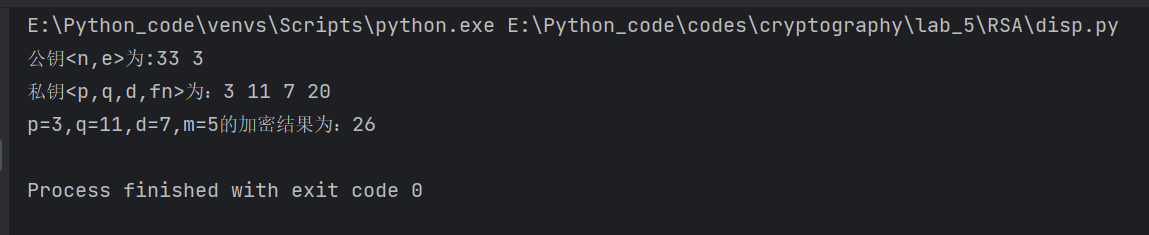
\includegraphics[width=13cm]{RSA_result1.png}
                \bottomcaption{\xiaowuhao{测试算法1运行结果}}
            \end{figure}
            
        \subsubsection{实验(2)}
            设RSA密码的 e=3,n=33,C=9, 手工或编程计算明文M 程序代码如下所示
            \lstinputlisting[caption={测试算法2},captionpos=b,firstline=17,lastline=25]{E:/Python_code/codes/cryptography/lab_5/RSA/disp.py}
            已知n之后将n分解为3*11,可以得到fn=2*10,由此可以计算得到d的值,所以能够得到明文
            \begin{figure}[H]
                \centering
                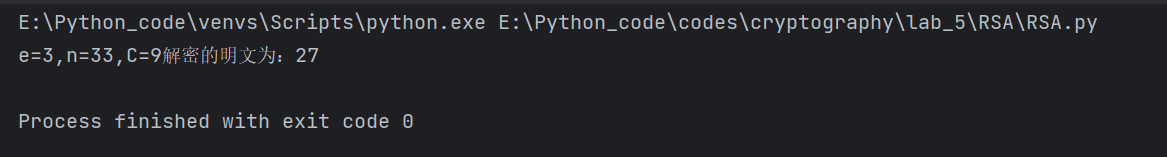
\includegraphics[width=13cm]{RSA_result2.png}
                \bottomcaption{\xiaowuhao{测试算法2运行结果}}
            \end{figure}

        \subsubsection{实验(3)}
            令p=17,q=11, e=7,试计算RSA密码其余参数,进一步对于m=88, 计算密文C 。程序代码如下所示
            \lstinputlisting[caption={测试算法3},captionpos=b,firstline=28,lastline=35]{E:/Python_code/codes/cryptography/lab_5/RSA/disp.py}
            首先调用init函数计算出d,n的值,然后再调用RSA\_encode函数对明文88进行加密。
            其余参数和加密结果如下图所示
            \begin{figure}[H]
                \centering
                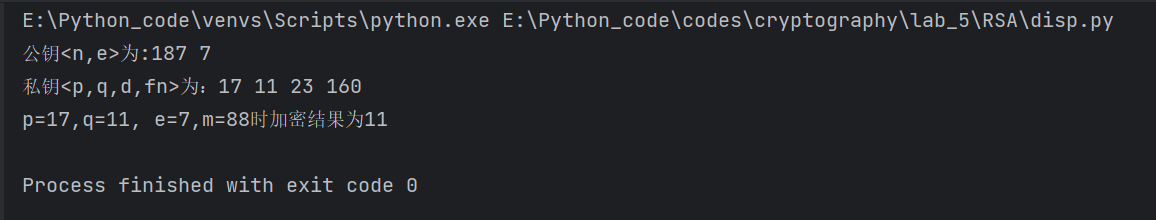
\includegraphics[width=13cm]{RSA_result3.png}
                \bottomcaption{\xiaowuhao{测试算法3运行结果}}
            \end{figure}

    \subsection{ELGamal密码}

        \subsubsection{密钥生成}
            用户随机地选取一个整数d作为自己的解密钥,然后计算$y=a^{d}mod\ p$的值作为公开加密钥。\par
            该过程的程序代码如下所示
            \lstinputlisting[caption={密钥生成},captionpos=b,firstline=27,lastline=41]{E:/Python_code/codes/cryptography/lab_5/ELGamal/ELGamal.py}
            在程序中如果没有题前设定p的值,则需要自动生成一个p,a和随机数d
\newpage
        \subsubsection{加密}
            加密过程为:用户随机选定一个整数k(1<k<p-1),首先计算$U=y^{k}mod\ p$然后计算$C_{1}=\alpha ^{k}mod\ p$与
            $C_{2}=UM\ mod\ p$将(C1,C2)作为加密得到的密文。\par
            加密程序如下所示
            \lstinputlisting[caption={ELGamal加密},captionpos=b,firstline=44,lastline=57]{E:/Python_code/codes/cryptography/lab_5/ELGamal/ELGamal.py}

        \subsubsection{解密}
            解密过程为:首先计算$V=C_{1}^{d}mod\ p$然后计算$M=C_{2}V^{-1}mod\ p$从而得到明文。\par
            解密程序如下所示
            \lstinputlisting[caption={ELGamal解密},captionpos=b,firstline=60,lastline=65]{E:/Python_code/codes/cryptography/lab_5/ELGamal/ELGamal.py}
            
        \subsubsection{实验}
            设p=19,m=17,构造一个ELGamal密码,并用它对m加密\par
            取$\alpha =2$,密钥d=765,随机数k=853加密得到的结果如下图所示
            \begin{figure}[H]
                \centering
                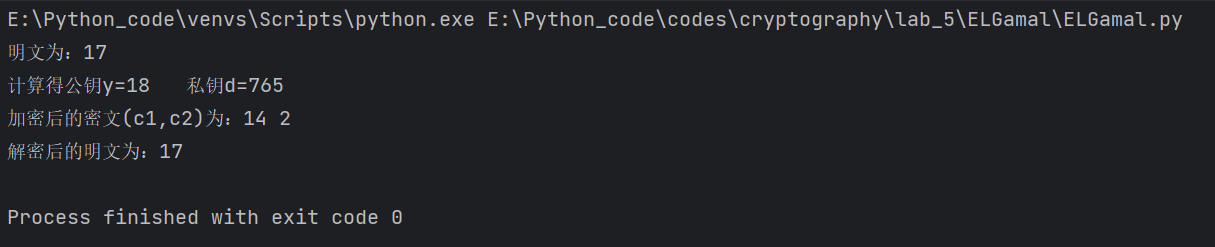
\includegraphics[width=13cm]{EL_result1.png}
                \bottomcaption{\xiaowuhao{测试算法1运行结果}}
            \end{figure}


        \subsubsection{实验(4)}
            设p=5,m=3,构造一个ELGamal密码,并用它对m加密
            取$\alpha =2$,密钥d=765,随机数k=853加密得到的结果如下图所示
            \begin{figure}[H]
                \centering
                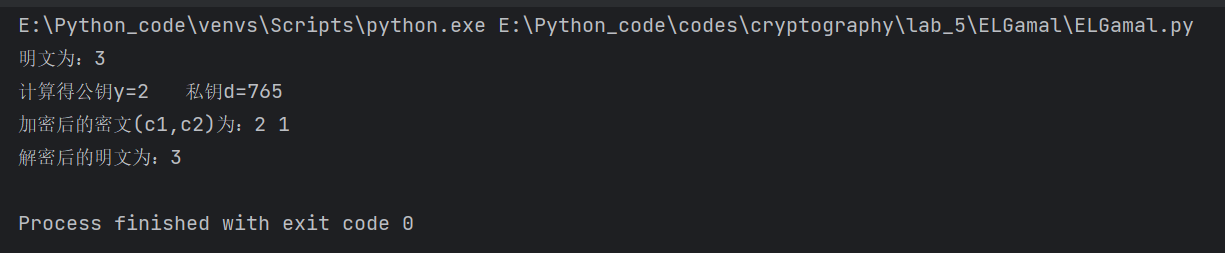
\includegraphics[width=13cm]{EL_result2.png}
                \bottomcaption{\xiaowuhao{测试算法2运行结果}}
            \end{figure}
\newpage
    \subsection{椭圆曲线密码}

        \subsubsection{求椭圆曲线所有解点(实验5)}
            编写求已知椭圆曲线和p的情况下所有的椭圆曲线的解点程序如下所示
            \lstinputlisting[caption={ELGamal解密},captionpos=b]{E:/Python_code/codes/cryptography/lab_5/SM2/椭圆曲线求解点.py}
            该程序使用穷举法首先遍历x的所有可能值,然后计算$y^{2}$接着,它再次遍历所有可能的y值,寻找使等式成立的 
            y。当找到这样的y时点(x,y)就是曲线上的一个解点。最后,程序返回曲线上的所有解点。\par
            将给出的椭圆曲线和p的值带入程序得到的运行结果为:
            \begin{figure}[H]
                \centering
                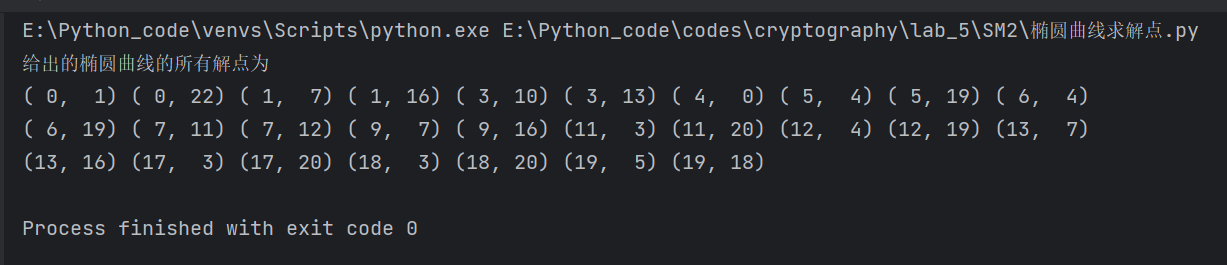
\includegraphics[width=13cm]{椭圆result1.png}
                \bottomcaption{\xiaowuhao{解点计算结果}}
            \end{figure}
        
        \subsubsection{SM2加密}
            SM2加密过程为:\par
            (1)定义一个随机数d作为用户的私钥,将用户的公钥定义为椭圆曲线上的P点,P=dG,G(x,y)是基点\par
            (2)用随机数发生器产生一个随机数k\par
            (3)计算椭圆曲线上的C1点C1=kG=(x1,x2)\par
            (4)计算椭圆曲线上的点S=$hP_{b}$的值,若S为无穷远点的话直接报错退出\par
            (5)计算椭圆曲线点(x2,y2)=$kP_{b}$\par
            (6)调用密钥派生函数KDF计算t的值,若计算出的t值为全0则返回(2)\par
            (7)调用二进制位上的异或函数,计算M与t的抑或结果保存到C2中\par
            (8)调用SM3-Hash密码杂凑函数根据x2,M,y2的拼接结果得到C3的值\par
            (9)将C1,C2,C3拼接起来作为密文输出\par
            SM2加密算法的算法流程图如下图所示
            \begin{figure}[H]
                \centering
                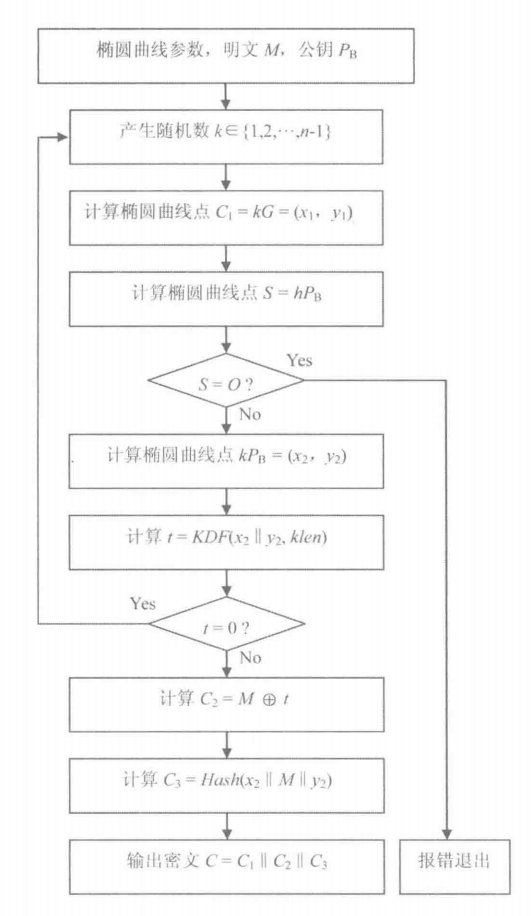
\includegraphics[width=8cm]{SM2加密流程.png}
                \bottomcaption{\xiaowuhao{SM2加密流程}}
            \end{figure}
            实现该过程的SM2加密算法如下所示
            \lstinputlisting[caption={SM2加密},captionpos=b,firstline=44,lastline=68]{E:/Python_code/codes/cryptography/lab_5/SM2/SM2.py}

        \subsubsection{SM2解密}
            SM2解密过程为:\par
            (1)验证C1是否满足椭圆曲线方程\par
            (2)计算椭圆曲线点S=hC1,若S为无穷远点则报错退出\par
            (3)计算(x2,y2)=$d_{B}C_{1}$\par
            (4)调用密钥派生函数KDF计算t的值,若计算出的t值为全0则报错\par
            (5)调用16进制字符串异或函数计算C2与t按位异或的结果,得出明文\par
            (6)调用SM3-Hash密码杂凑函数根据x2,计算得到的明文,y2得出的结果与C3相比,若两者不相等则报错。反之得到的明文为正确的明文\par
            SM2解密算法的算法流程图如下图所示
            \begin{figure}[H]
                \centering
                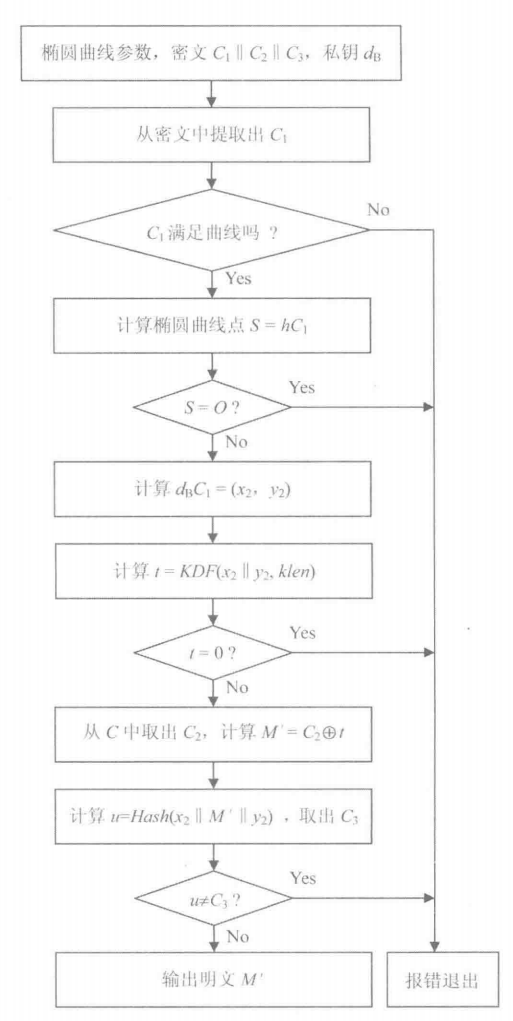
\includegraphics[width=8cm]{SM2解密流程.png}
                \bottomcaption{\xiaowuhao{SM2解密流程}}
            \end{figure}
            实现该过程的SM2解密程序如下所示
            \lstinputlisting[caption={SM2解密},captionpos=b,firstline=71,lastline=92]{E:/Python_code/codes/cryptography/lab_5/SM2/SM2.py}

        \subsubsection{KDF密钥派生函数}
            首先以每256比特为一组,循环生成足够的哈希数据,直到达到所需的密钥长度 klen。\par
            在每次循环中,使用 sm3hash 函数对 z 和 ct 的组合进行哈希处理。并将计数器 ct 转换为32位二进制形式,然后与 z 连接。\par
            之后将这个二进制字符串转换为十六进制字符串,用作 sm3hash 的输入。然后将哈希值加到 k 变量上,并将计数器 ct 加1。\par
            最后将之前生成的哈希字符串 k 转换为二进制形式,并确保其长度为256的倍数。返回所要求的位数\par
            密钥派生函数的实现代码如下所示
            \lstinputlisting[caption={KDF密钥派生},captionpos=b,firstline=33,lastline=41]{E:/Python_code/codes/cryptography/lab_5/SM2/SM2.py}
            
        \subsubsection{SM3-Hash密码杂凑函数}
            在SM2中所使用的Hash函数采用SM3中所使用的Hash函数,该函数首先将原始数据填充到适合的长度,以便进行处理。
            然后将填充后的数据分成多个固定大小的块。
            之后对每个数据块进行扩展,生成一系列新的数据。
            最后使用一系列复杂的数学运算,将扩展的数据压缩成一个固定长度的哈希值。\par
            本次实验中所调用的SM3-Hash密码杂凑函数代码如下所示
            \lstinputlisting[caption={密码杂凑函数},captionpos=b]{E:/Python_code/codes/cryptography/lab_5/SM2/sm3.py}
\newpage   
\section{实验结果与处理}

    \subsection{RSA加密}
        去掉所有的预制初始值之后运行RSA加密程序得到的结果如下图所示
        \begin{figure}[H]
            \centering
            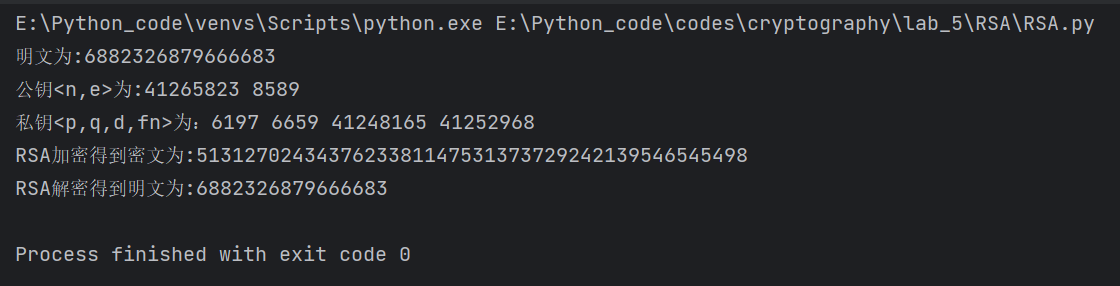
\includegraphics[width=13cm]{RSA_result.png}
            \bottomcaption{\xiaowuhao{RSA加解密结果}}
        \end{figure}

    \subsection{ELGamal加密}
        去掉所有的预制初始值之后运行ELGamal加密程序得到的结果如下图所示
        \begin{figure}[H]
            \centering
            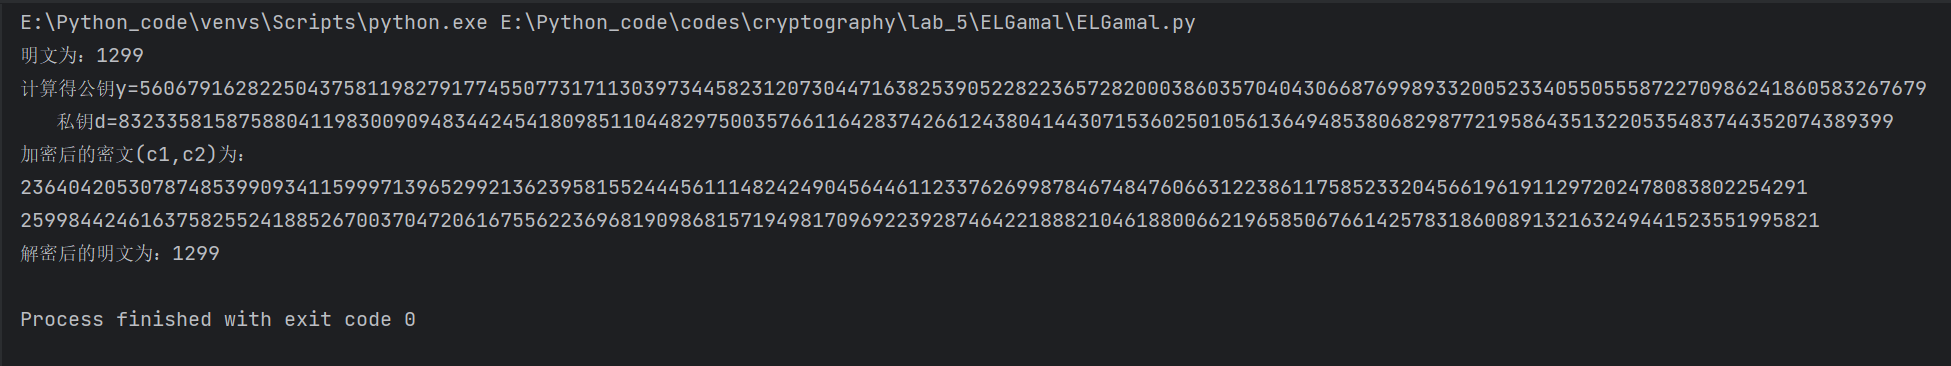
\includegraphics[width=13cm]{ELG_result.png}
            \bottomcaption{\xiaowuhao{ELGamal加解密结果}}
        \end{figure}

    \subsection{SM2加密}
        去掉所有的预制初始值之后运行SM2加密程序得到的结果如下图所示
        \begin{figure}[H]
            \centering
            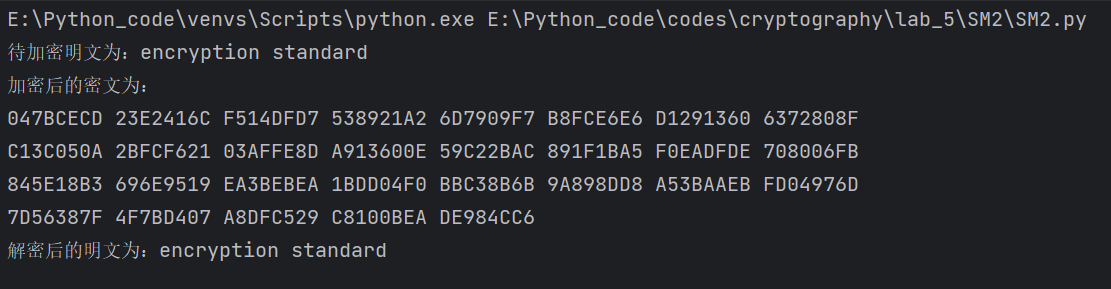
\includegraphics[width=13cm]{SM2_result.png}
            \bottomcaption{\xiaowuhao{SM2加解密结果}}
        \end{figure}


\section{分析与讨论}
    在这次密码学实验中,我深入了解了公钥密码学的核心原理,特别是RSA、ElGamal和椭圆曲线密码学等算法。
    通过编程实现这些算法,我更加清楚地认识到了它们在保护网络通信安全中的重要性。在实验过程中,我遇到了一些编程和逻辑上的挑战,通过不断的尝试和调试,
    我提高了解决问题的能力。总的来说,这次实验不仅提升了我的技术技能,也加深了我对网络安全重要性的理解。


\section{教师评语}

\end{document}
